\section{Create a Random Vertex}\label{appendix:random_gen}

Four random seeds are generated from the uniform distribution function: \texttt{RandFlat} in Class Library for High Energy Physics library (\texttt{CLHEP}).

One random seed is used for generating the time of the vertex: $t$ is a random variable following a uniform distribution in a range of $[100, 300]~ns$, say, $t\sim U(100,300)$.

Three random seeds are used for generating the position of the trial vertex: $\texttt{ran0}\sim U(0,1)$, $\texttt{ran1}\sim U(-1,1)$ and $\texttt{ran2Pi}\sim U(0,2\pi)$. 

Let $r=\sqrt[3]{\texttt{ran0}}*10000~mm$, $\phi=\texttt{ran2Pi}$, $\cos\theta=\texttt{ran1}$ and $\sin\theta=\sqrt{1-{\cos^2\theta}}$, then the trial position can be built in Cartesian coordinate system: $\vec{x}_{trial}=(r\sin\theta\cos\phi, r\sin\theta\sin\phi, r\cos\theta)$. This procedure ensures that a proper random position is generated inside a sphere with a radius of $10~m$.

For the trial direction, two random seeds are used. Each follows a uniform distribution: $\texttt{ranPi}\sim U(0,\pi)$ and $\texttt{ran2Pi}\sim U(0,2\pi)$. Then the trial direction is built as: $\vec{u}_{0}=(\cos\phi\sin\theta,\sin\phi\sin\theta,\cos\theta)$, with zenith angle $\theta=\texttt{ranPi}$ and azimuth angle $\phi=\texttt{ran2Pi}$.

Note that here the $\texttt{ranPi}$ and $\texttt{ran2Pi}$ are generated independently for the trial direction and they are not related to the vertex case.

\section{Levenberg-Marquardt Method}\footnote{This section refers to \cite{press2007numerical}.}\label{appendix:MRQ}

Levenberg-Marquardt (MRQ) method is a common routine for non-linear fitting. Let ${\bf a} = [a_0, a_1, ..., a_{M-1}]^T$ be an $M$-dimensional vector with $M$ unknown parameters to be fit, for example, $\bf a$ is an event vertex with 4 parameters: ${\bf a}=[x,y,z,t]^T$.

A $\chi^2$ merit function with the unknown parameter vector $\bf a$ can be built and by minimizing the function, the best-fit $\bf a$ can be found.

The $\chi^2(\bf a)$ can be approximately expanded into a quadratic form of Taylor-series:
\begin{equation} \label{eq:1}
\chi^2({\bf a})\simeq \gamma-{\bf d\cdot a}+\frac{1}{2}{\bf a\cdot D\cdot a},
\end{equation}
where $\gamma$ is a $M$-dimension constant vector around $\bf a$, $\bf d$ is a $M$-dimension vector and $\bf D$ is a $M\times M$ Hessian matrix.

To find a ${\bf a}_{min}$ so that a $\min\chi^2({\bf a}_{min})$ is reached, in computing science we usually use iteration steps: 
\begin{equation} \label{eq:2}{\bf a}_{min}={\bf a}_{cur}+D^{-1}[-\nabla\chi^2({\bf a}_{cur})],\end{equation} 
where ${\bf a}_{cur}$ is the current trial value of $\bf a$ and we assume matrix $\bf D$ is invertible. The ${\bf a}_{cur}$ thus jumps onto ${\bf a}_{min}$. 

According to the definition of a $\chi^2$ merit function, it can be written out explicitly as:
\begin{equation}
\chi^2({\bf a})=\sum_{i=0}^{N-1}[\frac{y_i-y(x_i|{\bf a})}{\sigma_i}]^2,
\end{equation}
and with the same Taylor expansion, the quadratic form is written as:
\begin{equation}\label{eq:3}
\chi^2({\bf a})\approx\chi^2({\bf a}_{cur})+\sum_k\frac{\partial \chi^2({\bf a}_{cur})}{\partial \alpha_k}\delta\alpha_k+\frac{1}{2}\sum_{kl}\frac{\partial^2\chi^2({\bf a}_{cur})}{\partial\alpha_k\partial\alpha_l}\delta\alpha_k\delta\alpha_l, 
\end{equation}
where the first derivatives are:
\begin{equation}\label{eq:4}
\frac{\partial \chi^2}{\partial a_k}=-2\sum_{i=0}^{N-1}[\frac{y_i-y(x_i|{\bf a})}{\sigma_i}]\frac{\partial y(x_i|{\bf a})}{\partial a_k}, k = 0,1,...,M-1,
\end{equation}
and the second derivatives are:
\begin{equation}\label{eq:5}
\frac{\partial^2 \chi^2}{\partial a_k\partial a_l}=2\sum_{i=0}^{N-1}\{\frac{\partial y(x_i|{\bf a})}{\partial a_k}\frac{\partial y(x_i|{\bf a})}{\partial a_l}-[y_i-y(x_i|a)]\frac{\partial^2 y(x_i|{\bf a})}{\partial a_k\partial a_l}\}, k = 0, 1, ..., M-1.
\end{equation}

Let $\beta_k\equiv-\frac{1}{2}\frac{\partial\chi^2}{\partial a_k}, \alpha_{kl}\equiv \frac{1}{2}\frac{\partial^2\chi^2}{\partial a_k\partial a_l}$, then the factor of 2 is removed. The $\alpha_{kl}$ is defined as the curvature matrix and ${\bf \alpha}=\frac{1}{2}{\bf D}$, which implies that it is the half of the Hessian matrix.

From \ref{eq:2}, we have: $D({\bf a}_{min}-{\bf a}_{cur}) = [-\nabla\chi^2({\bf a}_{cur})]\implies 2{\bf\alpha\delta a}= 2{\bf\beta}$. The \ref{eq:2} is now transformed into a systems of linear equations:
\begin{equation}\label{eq:6}
\sum_{l=0}^{M-1}\alpha_{kl}\delta a_l = \beta_k,
\end{equation} where $\delta a_l$ is 
a varying amount added to the current value of parameter for the next iteration. 

The main task now is to calculate $\alpha_{kl}$ and $\beta_k$ and then solve for $\delta a_l$ in \ref{eq:6}. Once $\delta a_l$ is solved, we can vary the current trial or approximate values of ${\bf a}_{cur}$ and let it go close to or reach the ${\bf a}_{min}$.

If we consider the method of steepest descent: ${\bf a}_{next}={\bf a}_{cur}-\mathrm{const}\cdot\nabla\chi^2({\bf a}_{cur})$, where $\mathrm{const}$ is a constant, then the $\delta a_l$ is solved by: 
\begin{equation}\label{eq:7}
\delta a_l=\mathrm{const}\cdot \beta_l, 
\end{equation}
where no Hessian matrix is needed.

In the MRQ method, in order to solve for $\delta a_l$, the detailed calculation of ${\bf D}^{-1}$ in \ref{eq:2} and the simplified calculation of steepest descent in \ref{eq:7} are combined and a smooth transition between \ref{eq:2} and \ref{eq:7} is considered.

In \ref{eq:7}, the $\mathrm{const}$ describes the distance or magnitude of how far the parameter should go along the gradient $\beta_l$. From dimensional analysis, since $\beta_k\equiv-\frac{1}{2}\frac{\partial\chi^2}{\partial a_k}$ and $\chi^2$ is a non-dimensional number, $[\beta_l]=[1/a_l]$. Then from \ref{eq:7}, $[\mathrm{const}]=[a^2_l]$. The $\mathrm{const}$ has the same dimension to the term $1/\alpha_{ll}= 1/(\frac{1}{2}\frac{\partial^2\chi^2}{\partial a_l\partial a_l})$, i.e., the diagonal elements in the curvature matrix. A bridge between \ref{eq:2} and \ref{eq:7} is thus built. The diagonal elements in the curvature matrix can control the magnitude of the $\mathrm{const}$, tells how far the parameter should go along the gradient. 

Then \ref{eq:7} can be written as:
\begin{equation}\label{eq:8}
\delta a_l = \frac{1}{\lambda \alpha_{ll}}\beta_l~or~\lambda \alpha_{ll}\delta a_l = \beta_l, 
\end{equation} 
where $\alpha_{ll}$ is written in a form of $\alpha_{ll}=\sum_{i=0}^{N-1}\frac{1}{\sigma^2_i}[\frac{\partial y(x_i|{\bf a})}{\partial a_l} \frac{\partial y(x_i|{\bf a})}{\partial a_l}]$ to ensure that $\alpha_{ll}$ is always positive; a fudge factor $\lambda$ can be set to $\lambda \gg 1$ to avoid the case when the value of $\mathrm{const}$ is taken too large.

Compare \ref{eq:6} and \ref{eq:8}, if define a new curvature matrix $\alpha'$ as $\alpha'_{jj}\equiv (1+\lambda)\alpha_{jj}$ (for diagonal  elements) and $\alpha'_{jk}\equiv \alpha_{jk}~~~(j\neq k)$ (for non-diagonal elements), these two equations can be combined into one: 
\begin{equation}\label{eq:10}
\sum_{l=0}^{M-1}\alpha'_{kl}\delta a_l = \beta_k
\end{equation}

From the definition of $\alpha'$, if $\lambda$ takes a large value, $\alpha'$ is dominated by diagonal elements, then \ref{eq:10} is close to \ref{eq:8}; while if $\lambda\to0$,  \ref{eq:10} is close to \ref{eq:6}.

The algorithm of the MRQ method requires a reasonable start value (first guess) of the fitting parameter $\bf a$ and a reasonable preset value of $\lambda$ (usually take $\lambda$ = 0.001). 
The iteration loop of the algorithm is: calculate the value of $\chi^2({\bf a})$, solve for $\bf \delta a$ from \ref{eq:10} and then calculate $\chi^2({\bf a+\delta a})$. During this loop, the algorithm checks whether $\chi^2({\bf a+\delta a})\geq\chi^2({\bf a})$, if it is, $\lambda$ is increased by $\lambda=10\cdot\lambda$; if not, $\lambda$ is decreased by $\lambda=0.1\cdot\lambda$.  

The iteration loop is terminated when the change amount of the $\chi^2$ is negligible: if the loop calculates several $\chi^2$ values which are close to each other within a fit tolerance (\texttt{fTolerance}): $|\chi^2_{curren}-\chi^2_{previous}|<\texttt{fTolerance}$, the algorithm will consider the $\chi^2$ is minimized with a set of best-fit parameters. Here the termination condition of iterating the $\chi^2$ value to convergence to the machine
accuracy or to the roundoff limit is not used, since $\chi^2$ is a statistical quantity rather than a solution of an equation. It is not statistical meaningful to vary the value of $\bf a$ to vary $\chi^2$ by a small amount $\ll 1$.

Once the minimum is reached, $\lambda$ is set to 0 and then the estimated covariance matrix of the standard errors in the fitted $\bf a$ can be calculated as: $C\equiv {\bf \alpha^{-1}}$.

The MRQ method is the core algorithm in the \texttt{MP fitter} framework for likelihood fitting. A few fitter setting parameters relating to the method can be optimized in practice. These parameters are:
\begin{itemize}
	\item fit tolerance: \texttt{fTolerance}, which is set for $|\chi^2_{curren}-\chi^2_{previous}|<\texttt{fTolerance}$.
	\item the number of good fits: \texttt{nGood}. The maximum number of the ``good fits'' required to be a valid result. This is to avoid the case when the MRQ minimizer finds a local minima instead of a global minima.
	\item the maximum iteration: \texttt{fMaxIter}. The allowed maximum number for looping the MRQ minimizer.
	\item the maximum number of start positions: \texttt{nStart}. If the start value does not give a valid result, the fitter will try another random start value. \texttt{nStart} is the maximum number of the start value the fitter is allowed to try.
\end{itemize}

Table.~\ref{table:MRQ_params} shows the optimized values of the fitter setting parameters for different phases. 

\begin{table}[ht]
	\centering
	\caption{\label{table:MRQ_params} Optimized fitter setting parameters for different physics phases.}	
	{\centering
		\begin{tabular*}{150mm}{c@{\extracolsep{\fill}}cccc}
			\toprule 
			SNO+ phase & \texttt{fTolerance} & \texttt{nGood} & \texttt{fMaxIter} & \texttt{nStart}\\
			\midrule
			water phase & 0.001 & 6 & 500 & 250\\
			partial-fill phase & 0.001 & 4 & 100 & 250\\
			scintillator phase & 0.001 & 4 & 100 & 250\\
			\bottomrule	
		\end{tabular*}
	}
\end{table}

A trade-off between the accuracy \& precision of the reconstructed results and the CPU time is considered. If increasing the \texttt{fTolerance} while decreasing the number of \texttt{nGood}, \texttt{fMaxIter} and \texttt{nStart}, the CPU time will decrease at costs of the fitter accuracy \& precision, and vice versa.

\section{Calculations of Derivatives of Likelihood Functions}\label{appendix:likelihoodCalcu}
The MRQ method requires the derivatives of the likelihood function. These derivatives can be calculated analytically in explicit mathematical forms.

The position difference is defined as $\vec{X}_{{\mathrm{diffCh}}} = \vec{X_0}-\vec{X}_{\mathrm{pmt}}$. Then the $TOF$ for the prompt Cherenkov light is $t_{\mathrm{Ch}}=|\vec{X}_{{\mathrm{diffCh}}}|/v_g$ and $L_{\mathrm{Ch}}=L(t_{\mathrm{Ch}})$.

Then it comes out for the water vertex case,
\begin{equation}
\frac{\partial L}{\partial t_0}=\frac{dL_{\mathrm{Ch}}}{dt_{\mathrm{Ch}}},
\end{equation}

\begin{equation}
\frac{\partial L}{\partial x}=\frac{\partial L_{\mathrm{Ch}}}{\partial t_{\mathrm{Ch}}}\frac{dt_{\mathrm{Ch}}}{\partial x}=-\frac{dL_{\mathrm{Ch}}}{dt_{\mathrm{Ch}}}\frac{X_{{\mathrm{diffCh}}}}{|\vec{X}_{{\mathrm{diffCh}}}|\cdot v_g},
\end{equation}

\begin{equation}
\frac{\partial L}{\partial y}=-\frac{dL_{\mathrm{Ch}}}{dt_{\mathrm{Ch}}}\frac{Y_{{\mathrm{diffCh}}}}{|\vec{X}_{{\mathrm{diffCh}}}|\cdot v_g},
\end{equation}

\begin{equation}
\frac{\partial L}{\partial z}=-\frac{dL_{\mathrm{Ch}}}{dt_{\mathrm{Ch}}}\frac{Z_{{\mathrm{diffCh}}}}{|\vec{X}_{{\mathrm{diffCh}}}|\cdot v_g},
\end{equation}

where the derivative $\frac{dL_{\mathrm{Ch}}}{dt_{\mathrm{Ch}}}$ can be calculated numerically from the timing $pdf$ saved as a binned histogram.

For the water direction case,
\begin{equation}
\frac{\partial L}{\partial\theta}=\frac{dL_{\mathrm{Ch}}}{d\cos\theta_{\mathrm{Ch}}}\frac{d\cos\theta_{\mathrm{Ch}}}{\partial\theta}
=\frac{dL_{\mathrm{Ch}}}{d\cos\theta_{\mathrm{Ch}}}\frac{d\vec{u}_0}{d\theta}\cdot\frac{\vec{X}_{{\mathrm{diffCh}}}}{|\vec{X}_{{\mathrm{diffCh}}}|},
\end{equation}

where $d\vec{u}_0/d\theta=(\cos\phi\cos\theta, \sin\phi\cos\theta, -\sin\theta)$ and 

\begin{equation}
\frac{\partial L}{\partial\phi}=\frac{dL_{\mathrm{Ch}}}{d\cos\theta_{\mathrm{Ch}}}\frac{d\cos\theta_{\mathrm{Ch}}}{d\phi}
=\frac{dL_{\mathrm{Ch}}}{d\cos\theta_{\mathrm{Ch}}}\frac{d\vec{u}_0}{d\phi}\cdot\frac{\vec{X}_{{\mathrm{diffCh}}}}{|\vec{X}_{{\mathrm{diffCh}}}|},
\end{equation} 
where $d\vec{u}_0/d\phi=(-\sin\phi\sin\theta, \cos\phi\sin\theta, 0)$. The derivative $\frac{dL_{\mathrm{Ch}}}{d\cos\theta_{\mathrm{Ch}}}$ can be calculated numerically from the PMT angular response $pdf$ saved as a binned histogram.

\section{Inversion of Hessian Matrix}
Matrix inversion is a frequent calculation when applying the MRQ method. In the \texttt{MP fitter}, the inversion of a $2\times 2$ Hessian matrix (usually used for direction reconstruction with two parameters) is calculated directly. For the higher dimension matrix, usually the $4\times 4$ matrix for vertex reconstruction, a \texttt{SDecompQRH} class is called for calculating the inversion matrix by using QR decomposition method\cite{press2007numerical}. This class was introduced by Jeff Tseng and it was modified from the \texttt{ROOT TDecompQRH} class\cite{TDecompQRH}. Compared to the ROOT version, its \texttt{Solve()} function was slightly modified for solving the matrix equation $Ax=b$, where $A = QR$ is composed of an orthogonal matrix $Q$ and an upper triangular matrix $R$. If the diagonal element in R is too small, instead of returning failure, the modified algorithm simply sets the corresponding x component to be 0. This allows an optimization for the MRQ method to continue in frequent cases when the matrix is singular.

\section{Likelihood Surfaces}\label{appendix:likelihoodSurface}

Fig.~\ref{likelihoodSurface} shows vertex likelihood surfaces produced by the MRQ method in the \texttt{MP water fitter}, for an typical {$^{16}$}N event (central run-100934, event GTID = 61836), projected on $X-Y$, $X-Z$ and $Y-Z$ planes. A clear global maxima gives the reconstructed vertex: $\vec{X}_{fit}=(-211.958, 503.399, 275.990)$ mm and $t_{fit}=217.039$ ns. 

\begin{figure}
	\centering
	%\subfigure[X-Y plane.]{\label{fig:1a}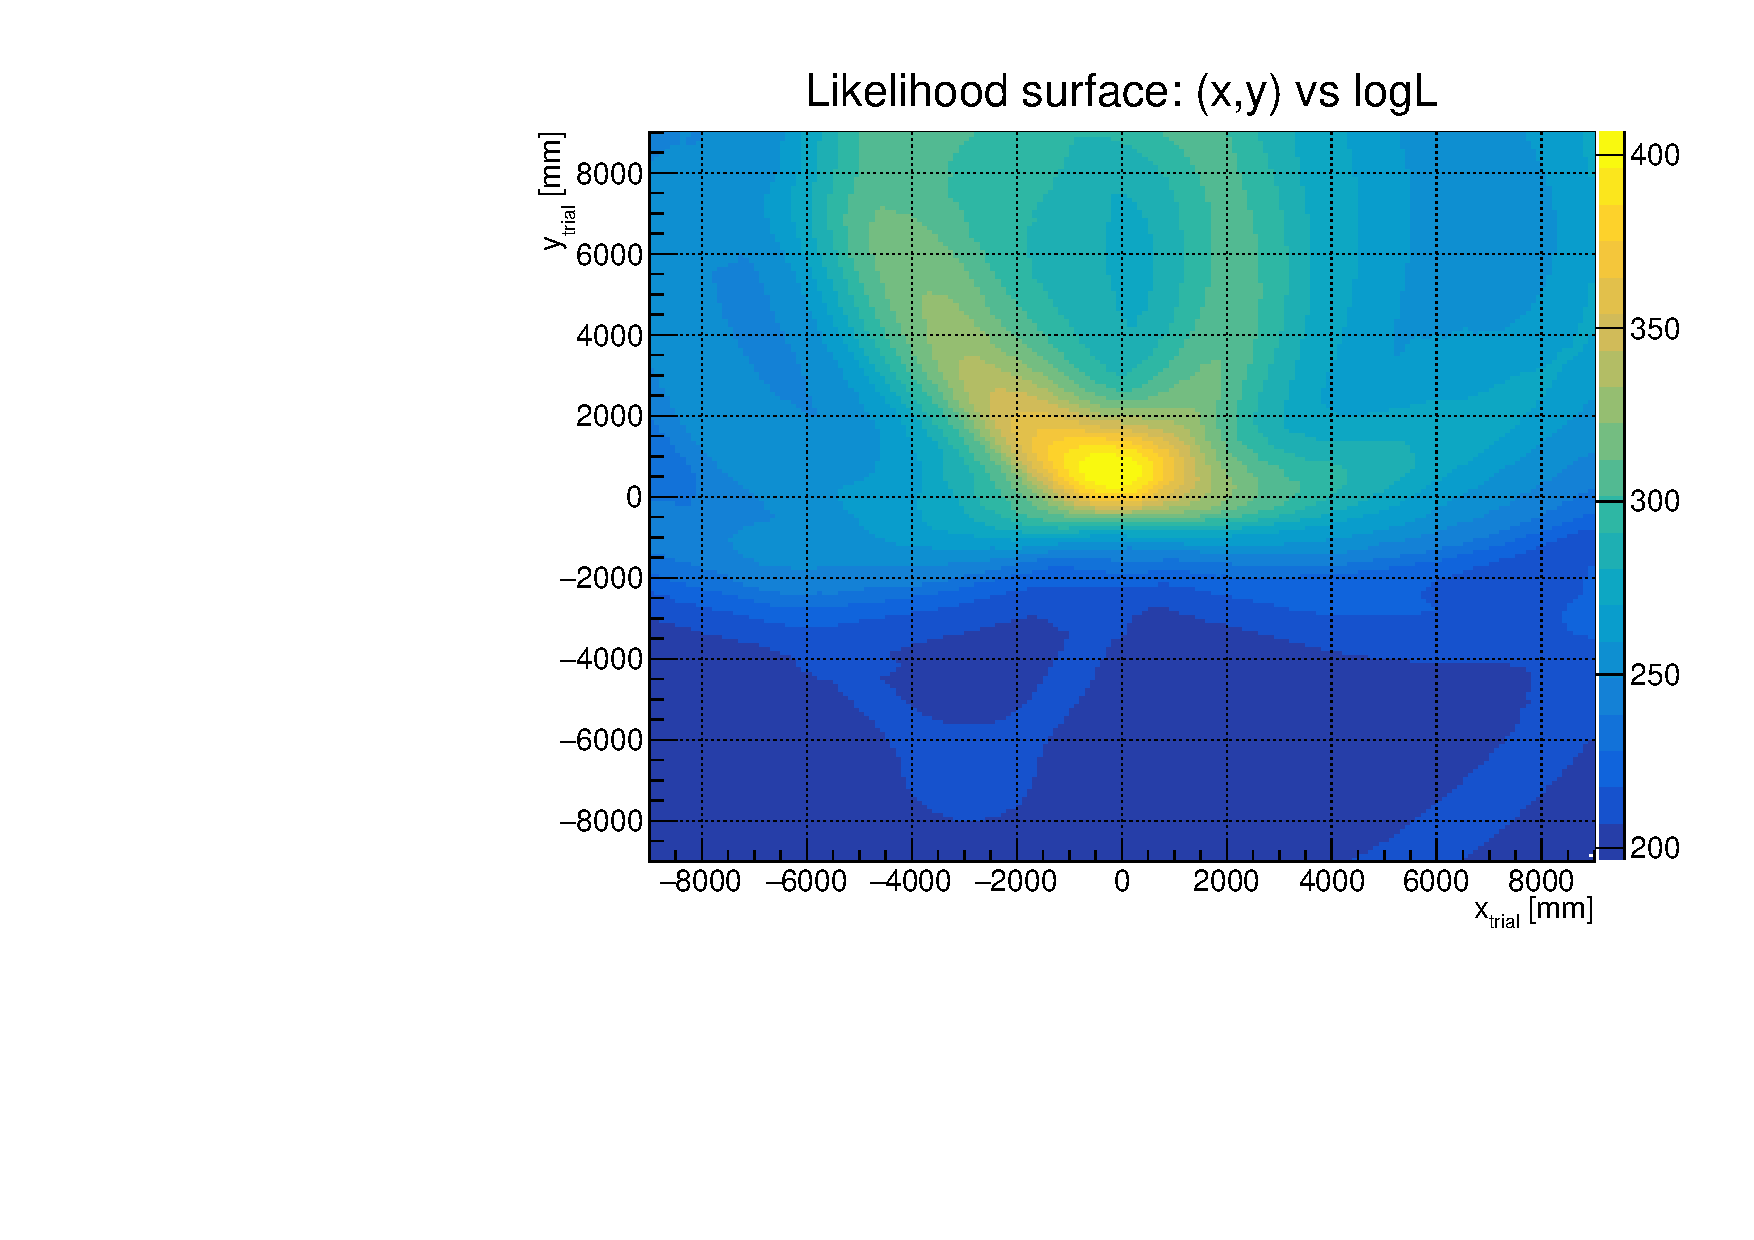
\includegraphics[width=65mm]{likelihoodSurface_xy.pdf}}
	%\subfigure[Y-Z plane.]{\label{fig:1b}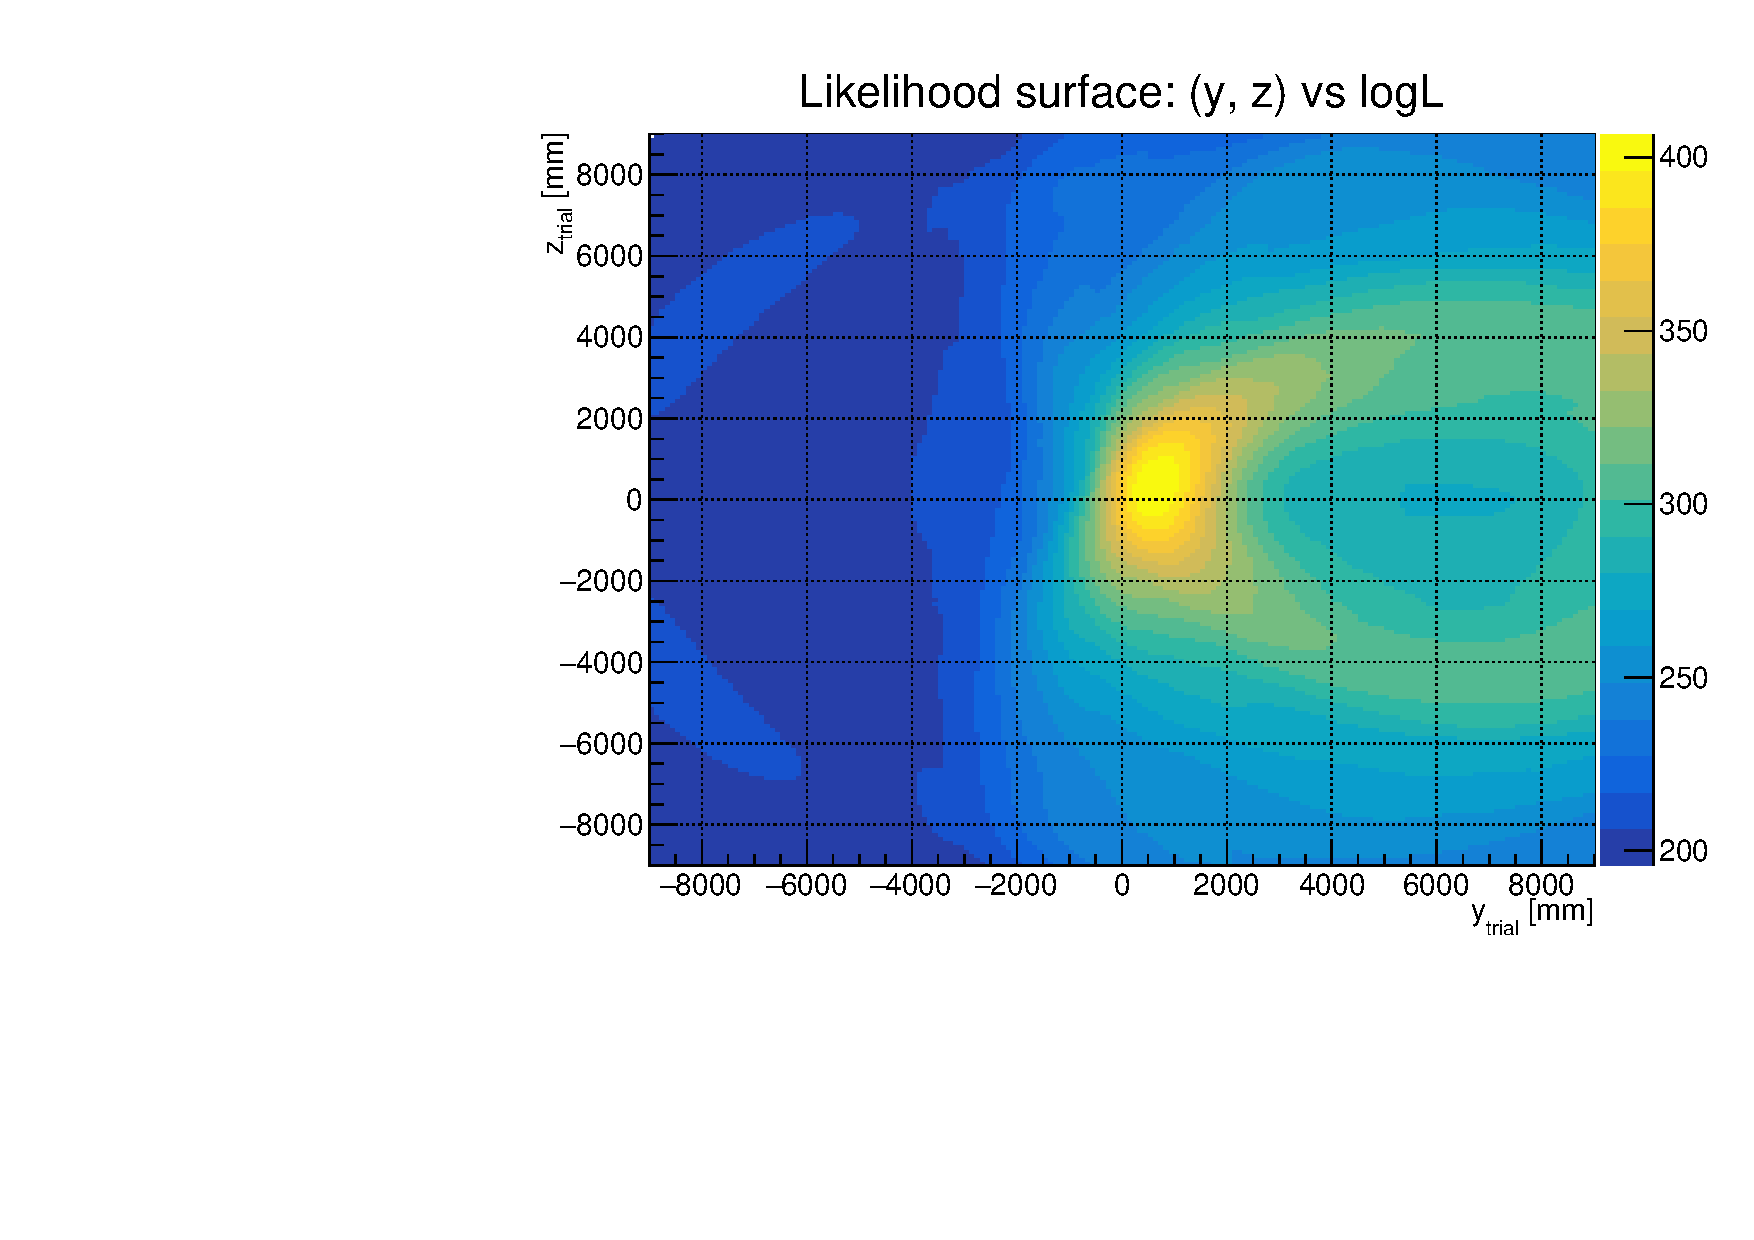
\includegraphics[width=65mm]{likelihoodSurface_yz.pdf}}
	%\subfigure[X-Z plane.]{\label{fig:1c}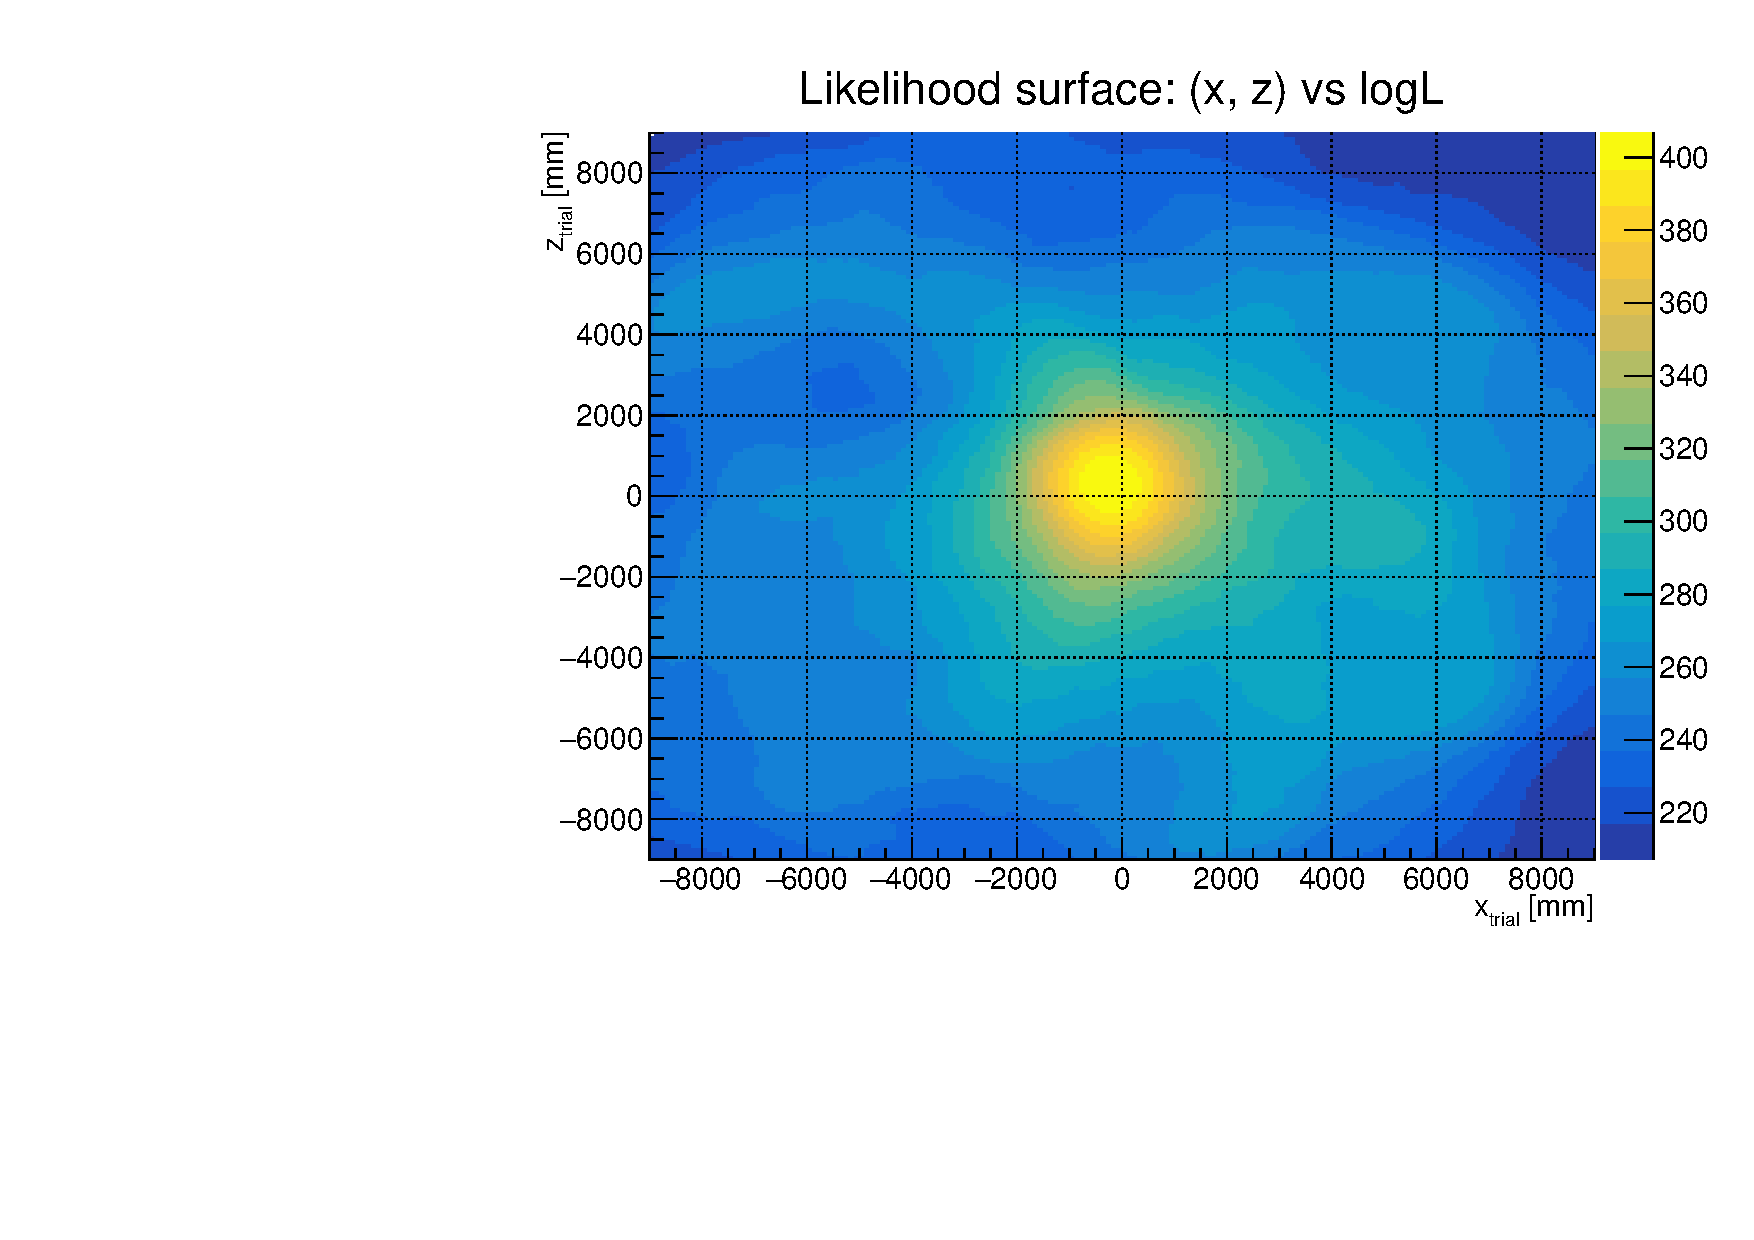
\includegraphics[width=65mm]{likelihoodSurface_xz.pdf}}
	\subfigure[X-Y plane.]{\label{fig:1a}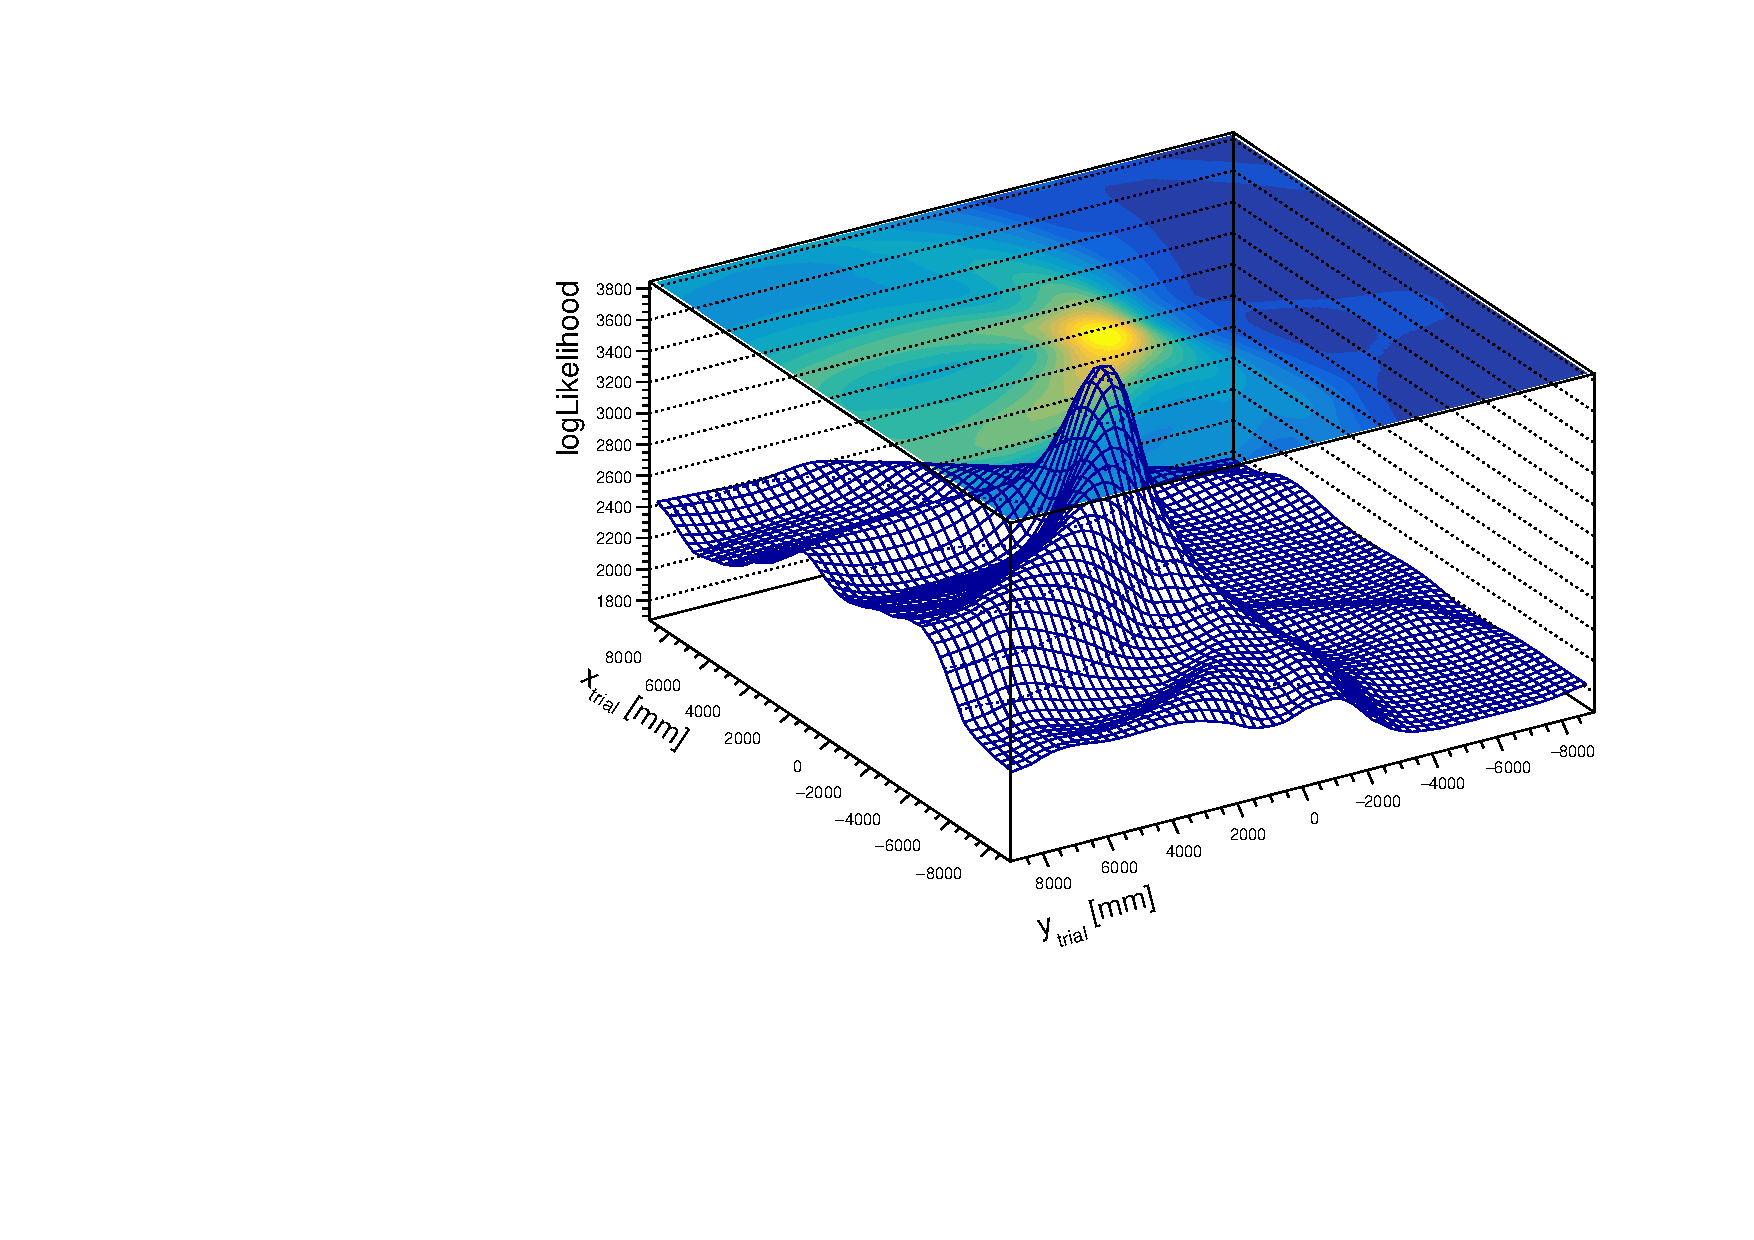
\includegraphics[width=75mm]{surf3_likelihoodXY.pdf}}
	\subfigure[Y-Z plane.]{\label{fig:1b}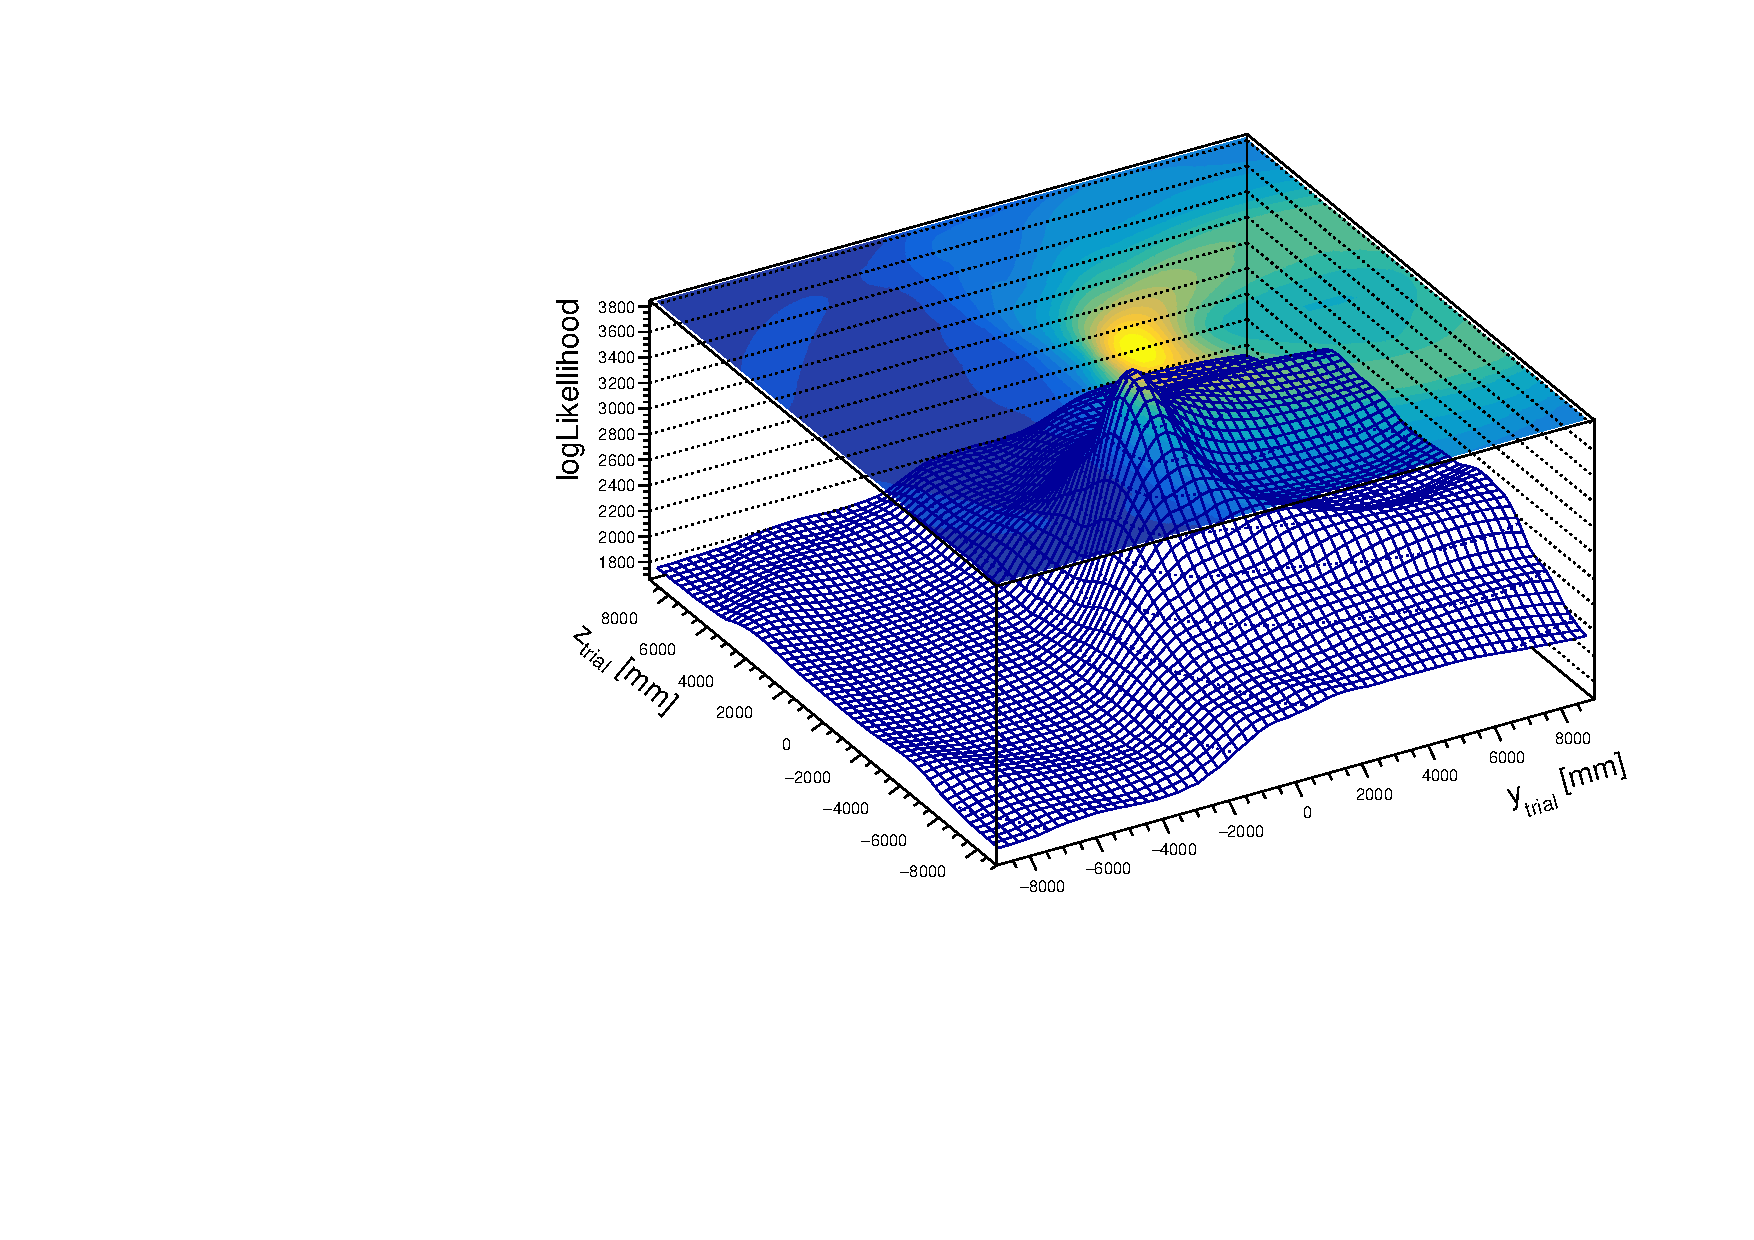
\includegraphics[width=75mm]{surf3_likelihoodYZ.pdf}}
	\subfigure[X-Z plane.]{\label{fig:1c}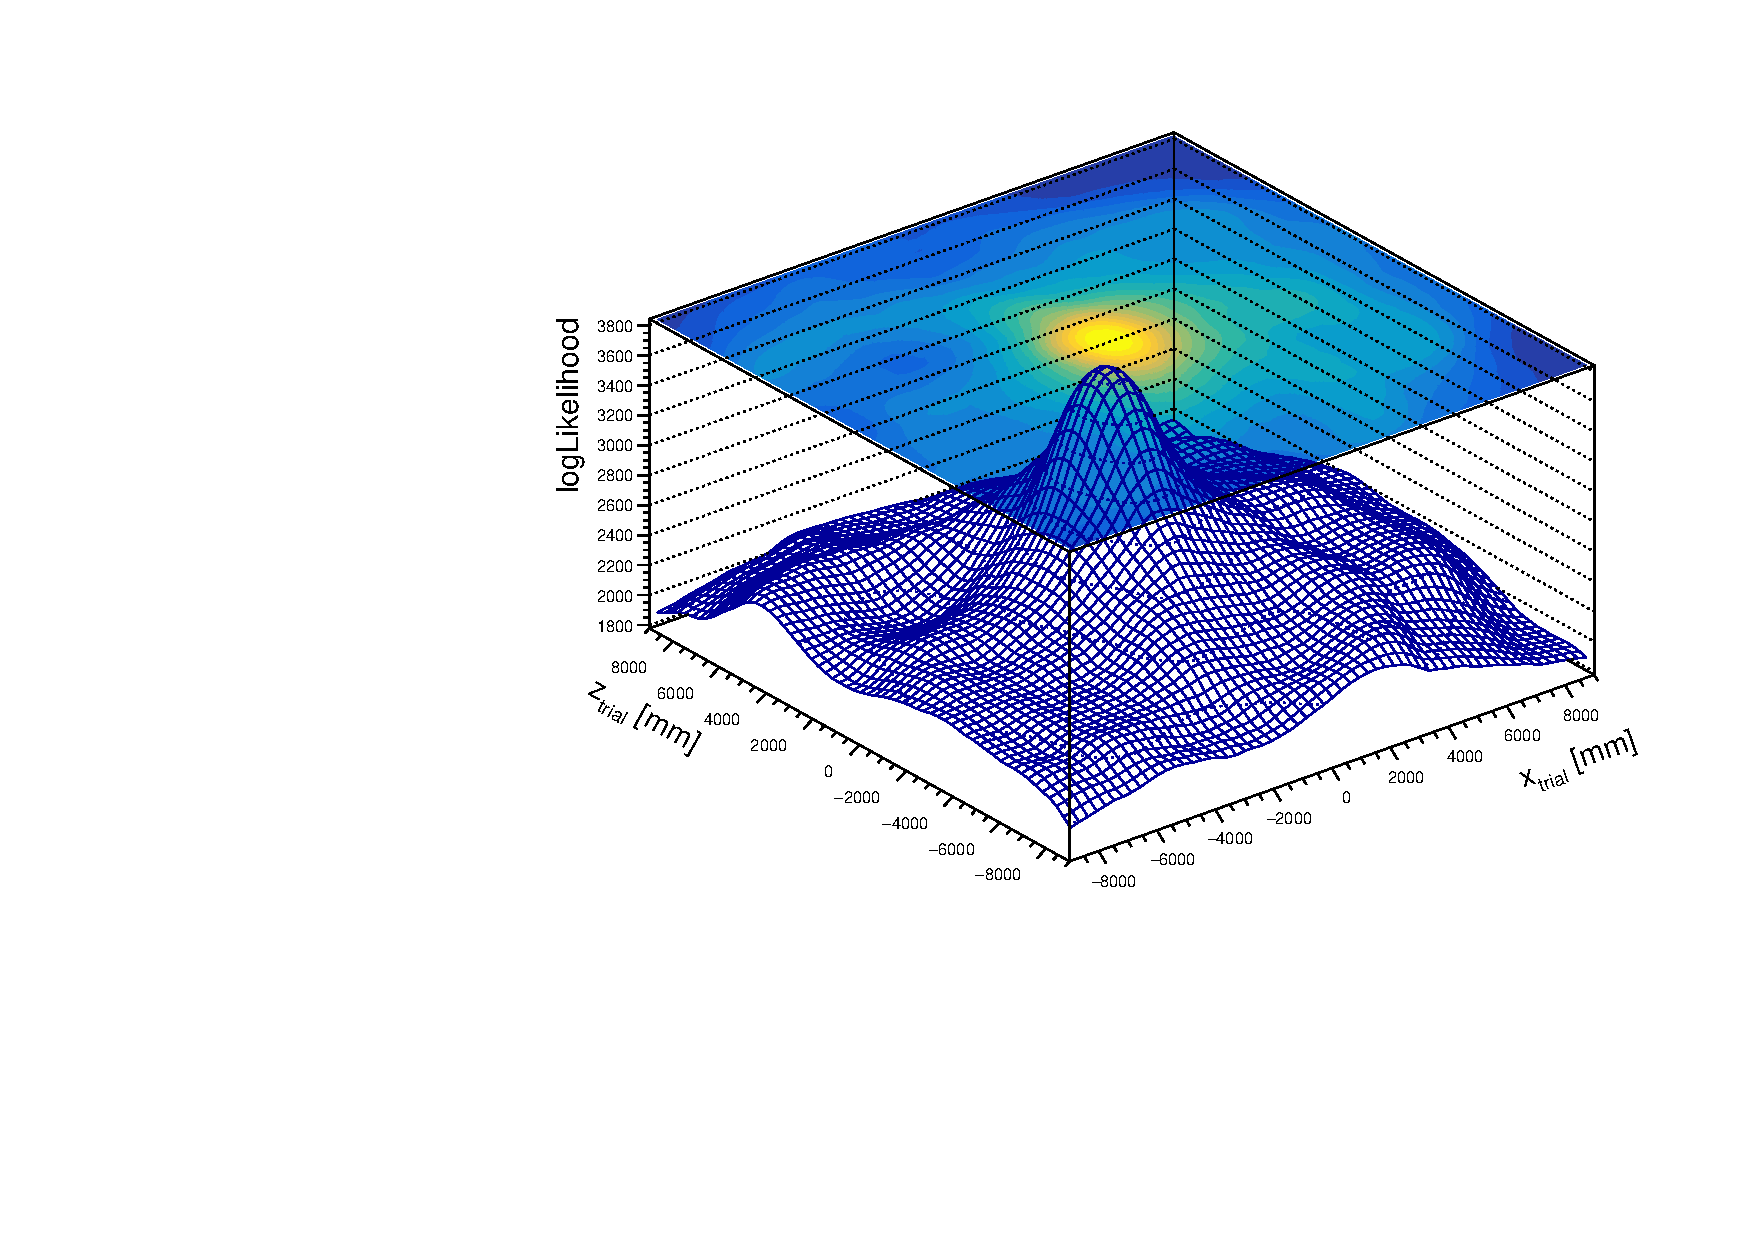
\includegraphics[width=75mm]{surf3_likelihoodXZ.pdf}}
	\caption{Likelihood surface of an {$^{16}$}N event projected on X-Y, Y-Z, X-Z planes. A clear global maxima is reached for the fitted vertex.}
	\label{likelihoodSurface}
\end{figure}

\begin{figure}
	\centering
	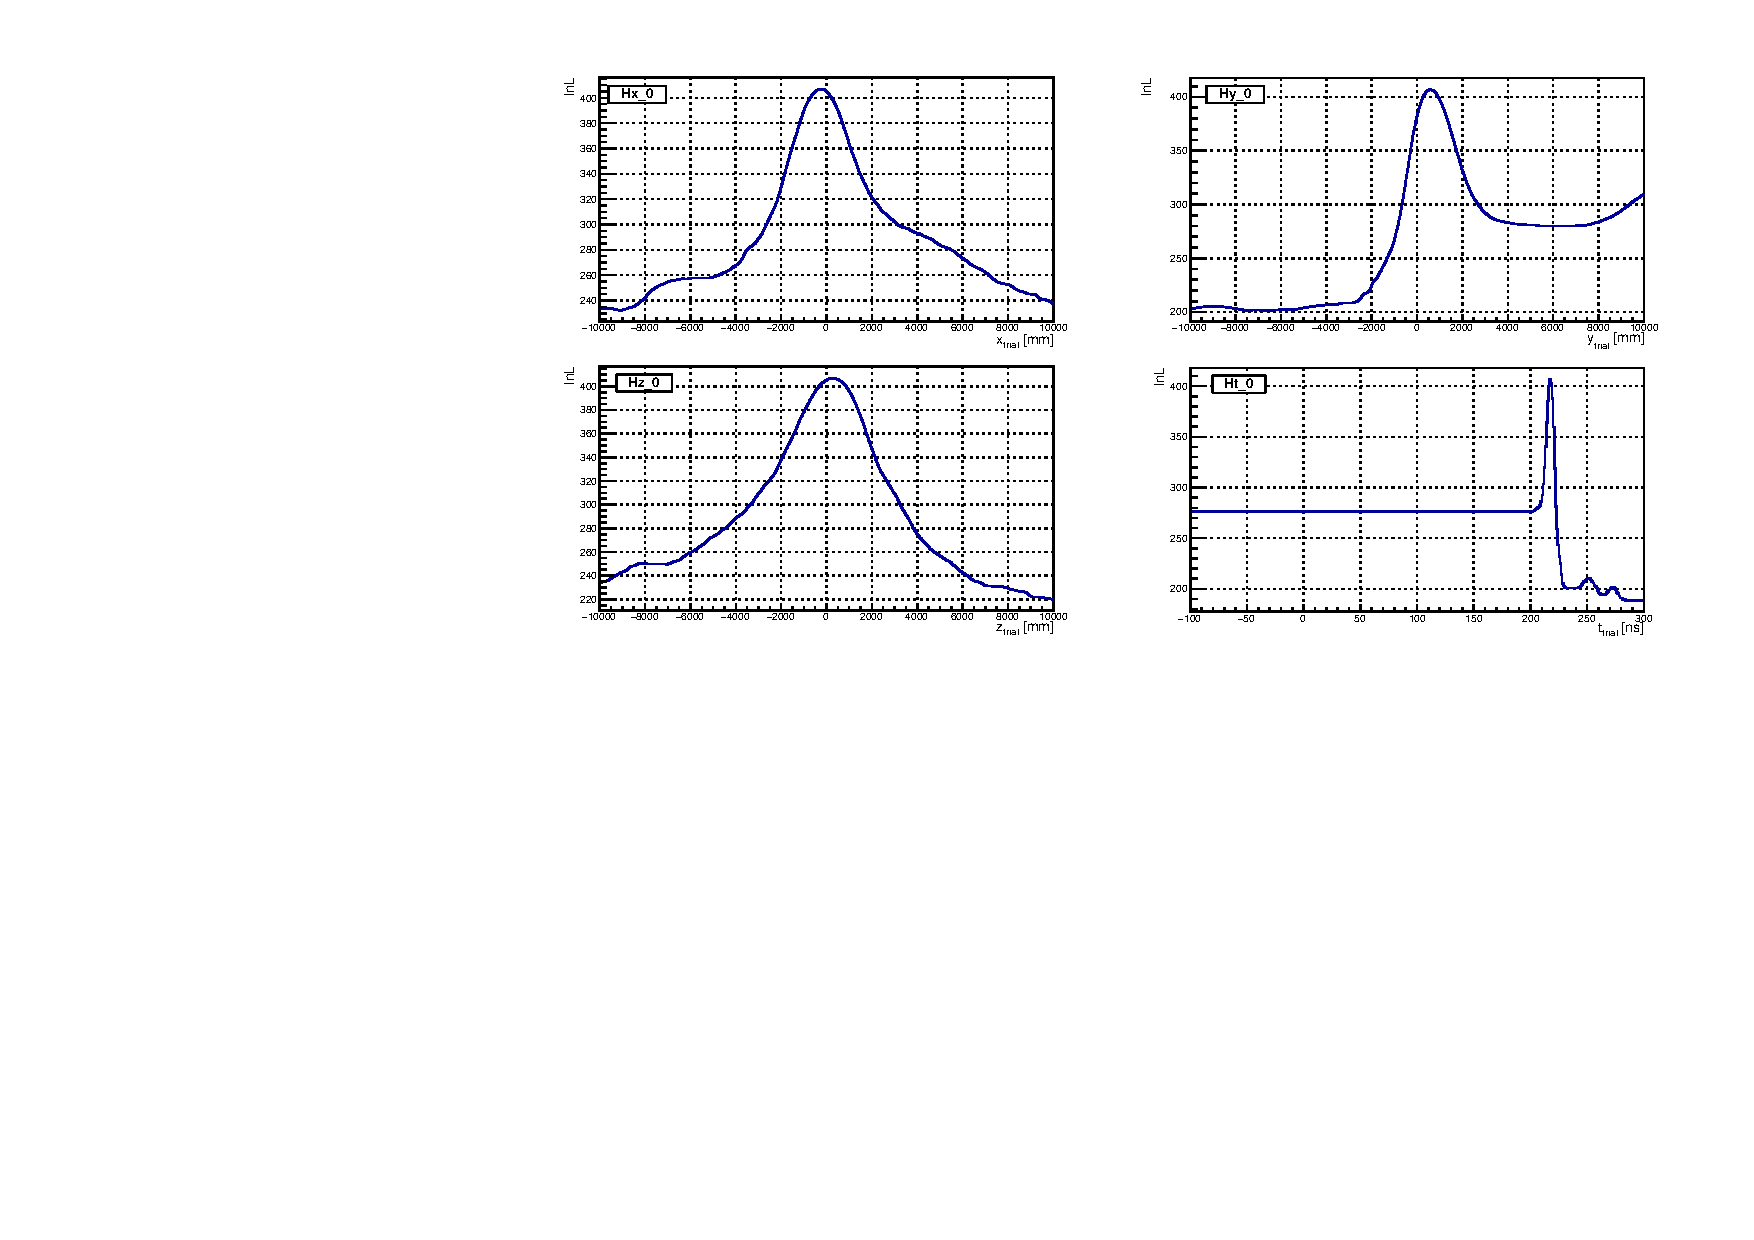
\includegraphics[width=160mm]{logL_xyzt.pdf}
	\caption{Likelihood surface of an {$^{16}$}N event projected on x, y, z, t-axis respectively.}
	\label{logLxyz}
\end{figure}

\begin{figure}
	\centering
	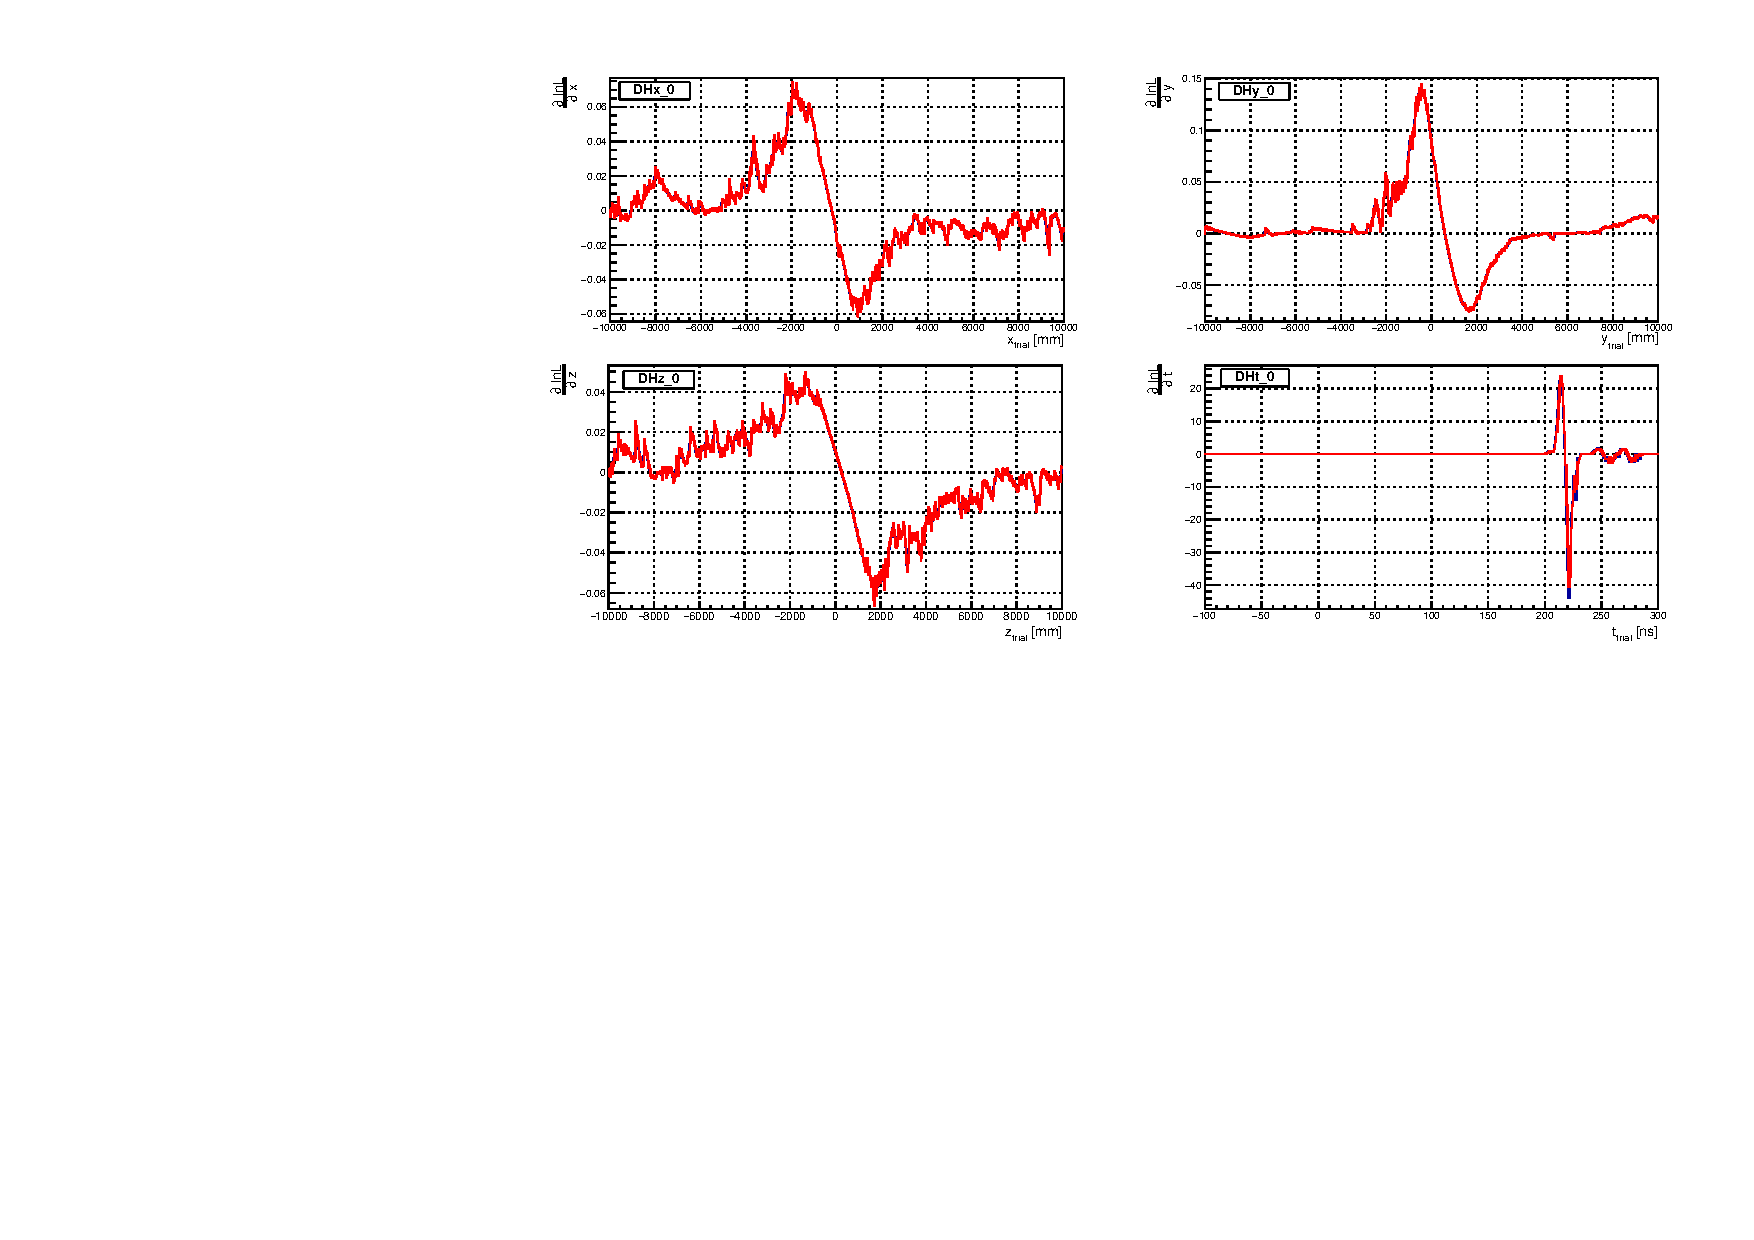
\includegraphics[width=160mm]{derivativeLogL_xyzt.pdf}
	\caption{Derivatives of $\ln L$ of an {$^{16}$}N event projected on x, y, z, t-axis respectively. The analytical derivatives (blue) are overlaid with numerical derivatives (red). They basically match with each other.}
	\label{derivative_logLxyz}
\end{figure}

\section{Detailed Light Path Calculations in the Multi-path Scint-water Fitter}\label{appendix:lightpath}
The following algorithm shows the detailed calculations for evaluating the light path in the scintillator regions. Each check steps are marked by number and if-conditions are marked by Latin letters (a, b or c). 

\begin{algorithm}
	First check the ray-sphere intersection (Equation.~\ref{eq:ray-cylinder}):\\
	If {$\Delta>0$}, 
	
	\hspace{2mm}(step. 1a) if $|\vec{x}_0|<r_{AV}$ (and $a_+>0>a_-$), check the ray-plane intersection:
	
	\hspace{4mm}(2a-a) if $a_3>0$, the ray-vector hits the interface plane: 
	
	\hspace{6mm}(3a-a-a) if $z_0<Z_{split}$ and $a_3<a_+$: $d_{sp,AV}=a_+-a_3$, see Fig.~\ref{lightpath_scintAV} (a).
	
	\hspace{6mm}(3a-a-b) if $z_0\geq Z_{split}$:
	
	\hspace{8mm}(4a-a-b-a) if $a_3<a_+$:  $d_{sp,AV}=a_3$, see Fig.~\ref{lightpath_scintAV} (b). 
	
	\hspace{8mm}(4a-a-b-b) if $a_3\geq a_+$:  $d_{sp,AV}=a_+$, see Fig.~\ref{lightpath_scintAV} (c).
	
	\hspace{4mm}(2a-b) if $a_3\leq0$:
	
	\hspace{6mm}(3a-b) if $z_0>Z_{split}$: $d_{sp,AV}=a_+$, see Fig.~\ref{lightpath_scintAV} (d).
	
	\hspace{2mm}(step. 1b) if $|\vec{x}_0|\geq r_{AV}$ (and $a_+>a_->0$), calculate the z position of the intersection point: $z_{\pm}=z_0+a_\pm\cdot(z_{PMT}-z_0)/|\vec{X}_{PMT}-\vec{X}_0|$:
	
	\hspace{4mm}(1-b-a) if $z_- \geq Z_{split}$ and $z_+\geq Z_{split}$: $d_{sp,AV} = a_+ - a_-$, see Fig.~\ref{lightpath_scintAV} (e).
	
	\hspace{4mm}(1-b-b) if $z_-< Z_{split}$ and $z_+> Z_{split}$ and $a_3>0$: $d_{sp,AV} = a_+ - a_3$, see Fig.~\ref{lightpath_scintAV} (f).
	
	\hspace{4mm}(1-b-c) if $z_->Z_{split}$ and $z_+<Z_{split}$ and $a_3>0$: $d_{sp,AV}= a_3 - a_-$, see Fig.~\ref{lightpath_scintAV} (g).
\end{algorithm}

\begin{figure}
	\centering
	{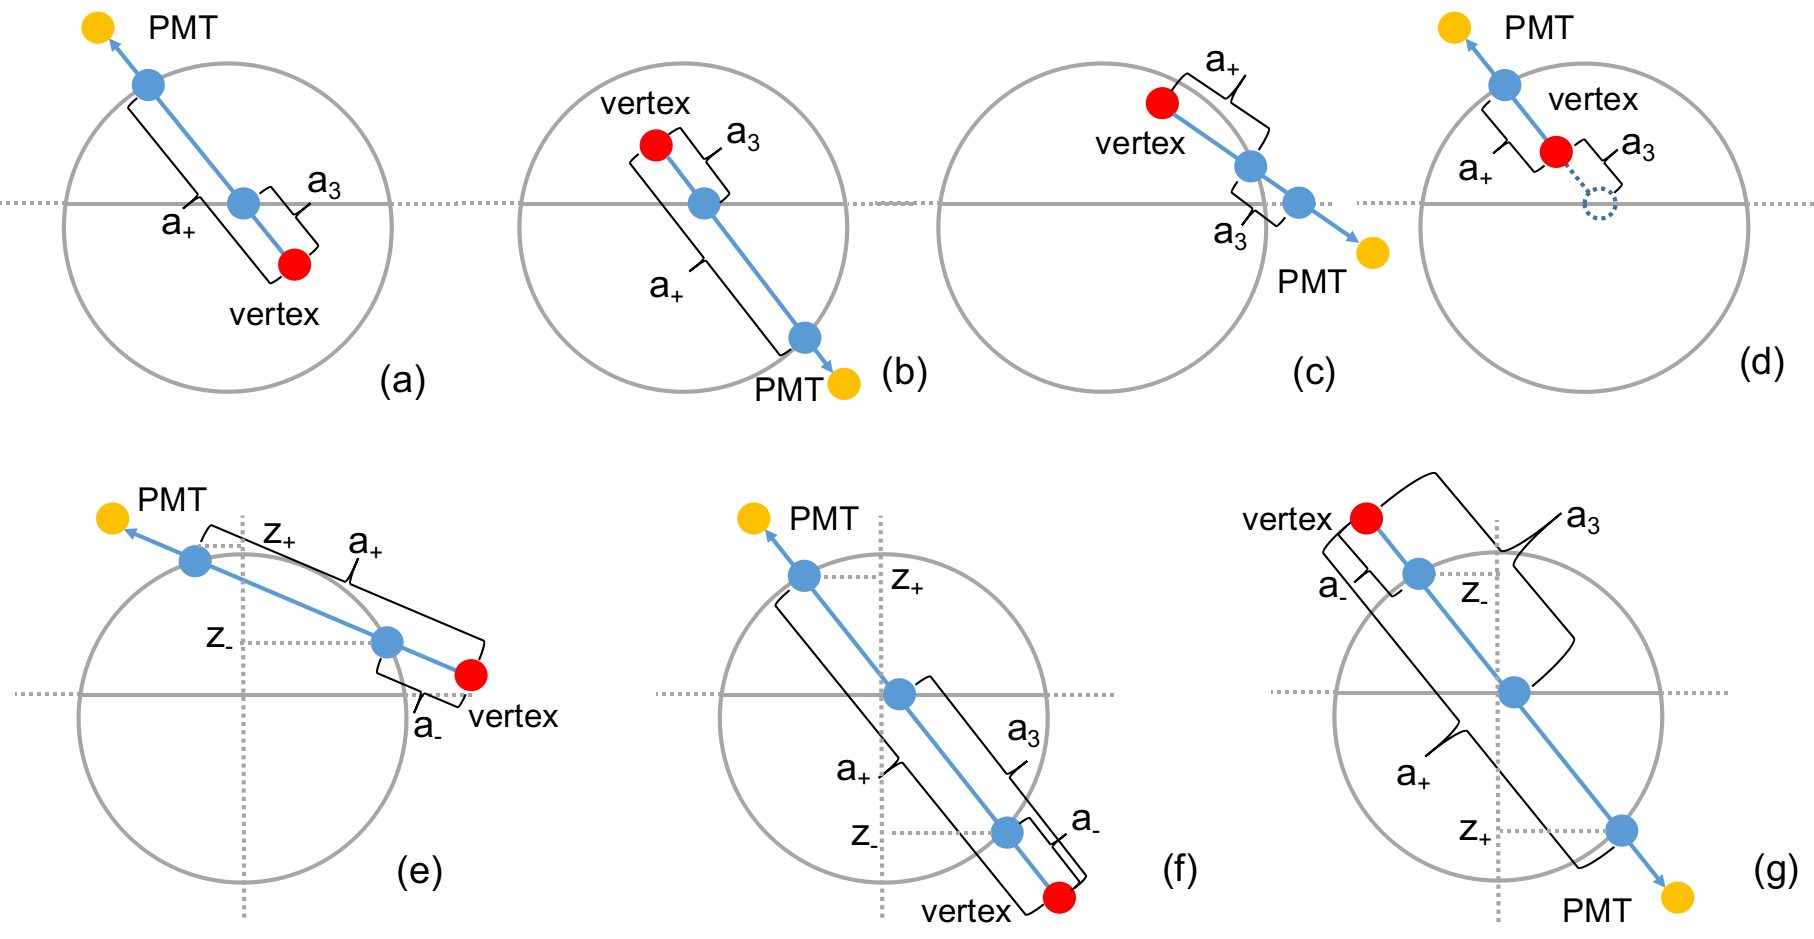
\includegraphics[width=130mm]{scintPathAV.png}}
	\caption{Layouts for the scintillator light paths inside the AV sphere.}\label{lightpath_scintAV}
\end{figure}

\begin{algorithm}
	
	First check the ray-cylinder intersection (Equation.~\ref{eq:ray-cylinder}):\\
	If {$\Delta_{neck}>0$}, 
	
	\hspace{2mm}(step. 1a) if $a'_+a'_-<0$ (event position is inside the cylinder), check the z position of the intersection point on neck, $z_+ = z_0 + a'_+u_z$: 
	
	\hspace{6mm}(2a-a) if $6108<z_+<8390~mm$ (in the valid neck region), then check the AV sphere:
	
	\hspace{8mm}(3a-a-a) if $|\vec{X}_0|\geq r_{AV}$: $d_{sp,neck}=a'_+$, see Fig.~\ref{lightpath_scintNeck} (a).
	
	\hspace{8mm}(3a-a-b) if $|\vec{X}_0|<r_{AV}$ and $a_+a_-<0$: $d_{sp,neck}=a'_+-a_+$, the light ray first hits the sphere inside the cylinder and then hits the cylinder, see Fig.~\ref{lightpath_scintNeck} (b). 
	
	\hspace{6mm}(2a-b) if $z_+<6108~mm$:
	
	\hspace{8mm}(3a-b) if $|\vec X_0|\geq r_{AV}$ and $6108<z_0<8390~mm$:
	
	\hspace{10mm}(4a-b) if $a_+>a_->0$: $d_{sp,neck}=a_-$, see Fig.~\ref{lightpath_scintNeck} (c).
	
	\hspace{2mm}(step. 1b) if $a'_+>a'_->0$ (event position is outside the cylinder), check the z position of the intersection point on neck, $z'_{\pm}=z_0+a'_\pm\cdot u_z$:
	
	\hspace{6mm}(2b-a) if $6108<z'_\pm-<8390~mm$, check the AV intersection:
	
	\hspace{8mm}(3b-a-a) if $a_\pm$ do not exit (never passes through AV), $d_{sp,neck}=a'_+ - a'_-$, see Fig.~\ref{lightpath_scintNeck} (d).
	
	\hspace{8mm}(3b-a-b) if $a_+>a_->0$, evaluate the z positions of the ray-sphere intersection points $z_\pm=z_0+a_\pm\cdot u_z$:
	
	\hspace{10mm}(4b-a-a) if $z_\pm\geq 6108~mm$: $d_{sp,neck}=a'_+ - a'_--(a_+-a_-)$, see Fig.~\ref{lightpath_scintNeck} (e). The path inside the sphere is subtracted to avoid duplicated calculation.
	
	\hspace{10mm}(4b-a-b) if $z_+<6108$ and $6108<z_-<8390~mm$:
	
	\hspace{12mm}(5b-a-b-a) if $a_+>a_->0$: $d_{sp,neck}=a_--a'_-$, see Fig.~\ref{lightpath_scintNeck} (f).
	
	\hspace{12mm}(5b-a-b-b) if $z_-<6108$ and $6108<z_+<8390~mm$:
	
	\hspace{14mm}in this case, either the event position is inside the sphere ($a_+a_-<0$), shown in Fig.~\ref{lightpath_scintNeck} (g), or outside the sphere ($a_+a_-<0$), shown in Fig.~\ref{lightpath_scintNeck} (h)), the path in neck is same: $d_{sp,neck}=a'_+ - a_+$.
\end{algorithm}


\begin{figure}
	\centering
	{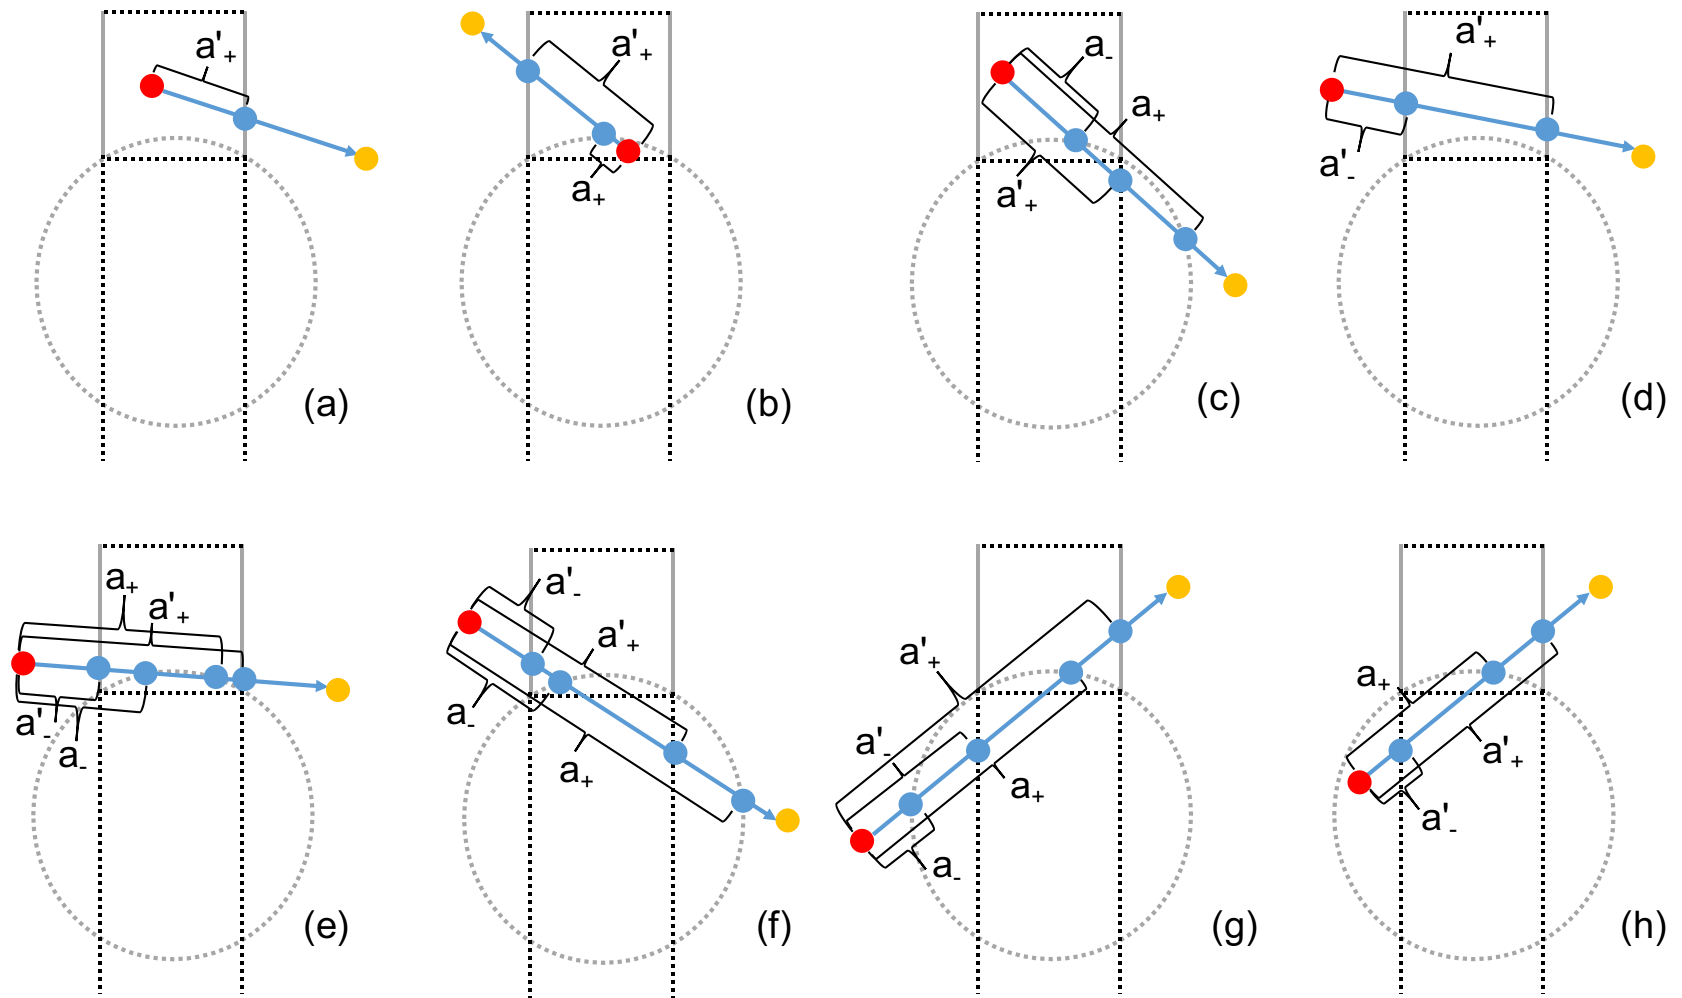
\includegraphics[width=130mm]{scintpathNeck.png}}
	\caption{Layouts of the scintillator light paths inside the neck cylinder.}\label{lightpath_scintNeck}
\end{figure}

%\[t_{transit}=(a_+-a_3)/v_{gr,scint}+[|\vec{X}_{\mathrm{pmt}}-\vec{X}_0|-(a_+-a_3)]/v_{gr,water}\]